\documentclass[12pt]{article}

\usepackage{breqn}
\usepackage[margin=1in]{geometry} 
\usepackage{amsmath,amsthm,amssymb,enumitem}
\usepackage[german,spanish,english]{babel}
\usepackage{tensor}
\usepackage{graphicx}
\usepackage{esint}
\usepackage[T1]{fontenc}
\usepackage{mathtools}
\usepackage{siunitx}
\newenvironment{ex}[2][Exercise]{\begin{trivlist}
\item[\hskip \labelsep {\bfseries #1}\hskip \labelsep {\bfseries #2.}]}{\end{trivlist}}

\newenvironment{sol}[1][Solution]{\begin{trivlist}
\item[\hskip \labelsep {\bfseries #1:}]}{\end{trivlist}}

\newcommand{\meq}{\overset{!}{=}}
\DeclarePairedDelimiter\bra{\langle}{\rvert}
\DeclarePairedDelimiter\ket{\lvert}{\rangle}
\DeclarePairedDelimiterX\brk[2]{\langle}{\rangle}{#1\,\delimsize\vert\,\mathopen{}#2}
\DeclareSIUnit\angstrom{\text {Å}}

%DECLARATION OF DELIMITERS%

\DeclarePairedDelimiter\vb{\lvert}{\rvert}
\DeclarePairedDelimiter\rb{(}{)}
\DeclarePairedDelimiter\sqrb{[}{]}
\DeclarePairedDelimiter\cb{\{}{\}}
\DeclarePairedDelimiter\ab{\langle}{\rangle}
\DeclarePairedDelimiter\db{\|}{\|}


\begin{document}
\noindent Richard Abele \hfill \today \\[30pt]
\centerline{ \Large{ \textbf{ Numerical Methods in Physics and Astrophyiscs }}}
\centerline{ \Large{ \textbf{ Problem Set 2 : Fractals Through Newton-Raphson }}}

\section{Working Principle}
\label{sec:principle}



To fulfill the necessary requirements for the assignment, the root finding program from the previous problem set is adapted to work with complex numbers and find the roots of a complex function. Two loops are then created to iterate what will be the pixels of a fractal image. 

During the execution of the program, the y-values are calculated in parallel for different x-values and stores in a buffer. This buffer is then written to a file. Some brief testing indicates that using OpenMP and some primitive parallelization yielded a performance improvement of about six to ten fold. 

Plotting the imaginary component of the root obtained or the number of iterations required to reach said root with a corresponding color map produces many wonderful images in the form of fractals. 

\section{Usage}
\label{sec:usage}


A program called \texttt{calc_fractal} is created after running \texttt{make} in the project directory. Running \texttt{./calc_fractal} uses the values in \texttt{lib/constants.c} to generate the desired data in \texttt{data/fractal_data.csv} in the format \(x_{0},y_{0},  \Re k\rb*{z}, \Im k \rb*{z}, \Re f \rb*{z}, \Im f \rb*{z}\), and \(\log_{10}\rb*{n}\) with \(n\) being the number of iterations needed . This counter and other parameters were set to 0 when a point did not converge. 

Additionally, one can use \texttt{./calc_fractal} with two points defining a viewing window in which the fractal data is calcualted (the default goes from (-2,-2) to (2,2)). In other words, one can write \texttt{./calc_fractal <p1_x> <p1_y> <p2_x> <p2_y>} with \texttt{p1} being the coordinates of the lower left corner and \texttt{p2} the coordinates of the top right corner. 

Fractals are then plotted with \texttt{gnuplot} using the \texttt{.gp} file in \texttt{plots/}. Images of he fractals can be found in the same \texttt{plots/} directoy with the formal \texttt{fractal_plot_<ID>_<Img Vers>} with the ID corresponding to an equation and the second parameter the image version. Images with an ID of 1 were experimental.

Please note that successfully plotting the data requires the deleting of \texttt{fractal_data.csv} from \texttt{/data} in order to create a new set of data. Additionally, one can change the \texttt{.gp} file in order to create images with different resolutions, output names, and dependent variables (either the \(\Im f\rb*{z}\) or \(\log_{10} n\)).

\section{Results}
\label{sec:results}

\subsection{First Function}
\label{subsec:first}



We will begin by observing the results obtained from plotting the first function:
\begin{align*}
	f\rb*{z} & =  z^{3} - 1 = 0 &\\
\end{align*}

     \begin{figure}[ht]
    \centering
    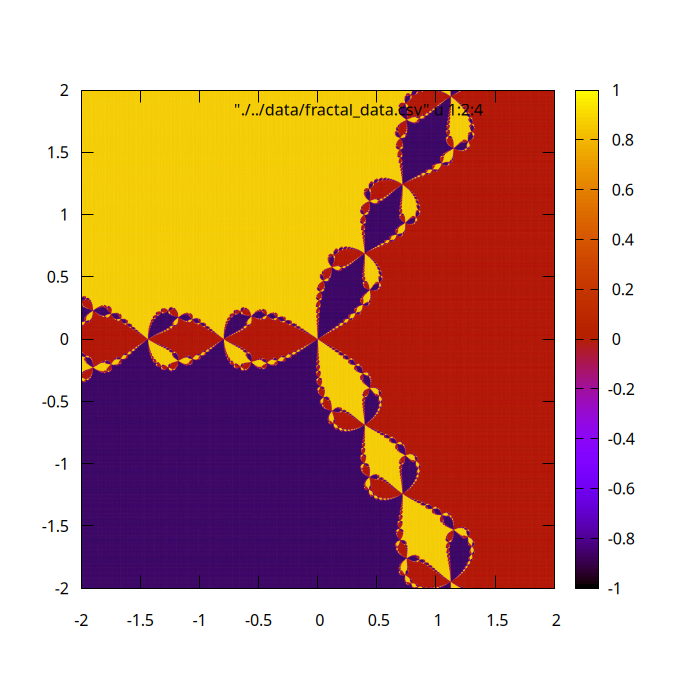
\includegraphics[width=0.75\textwidth]{./../problem04/plots/fractal_plot-02_01.png}
    \caption{\( \Im f\rb*{z}\) plotted on the complex plane from \(-2 -2i\) to \(2 + 2i\).}
    \label{fig:02_01}
\end{figure}

Note that the color scale on the right side of the image shows \(\Im f\rb*{z}\).

We then coninue by choosing a region with complex behavior and plotting two more images:

     \begin{figure}[ht]
    \centering
    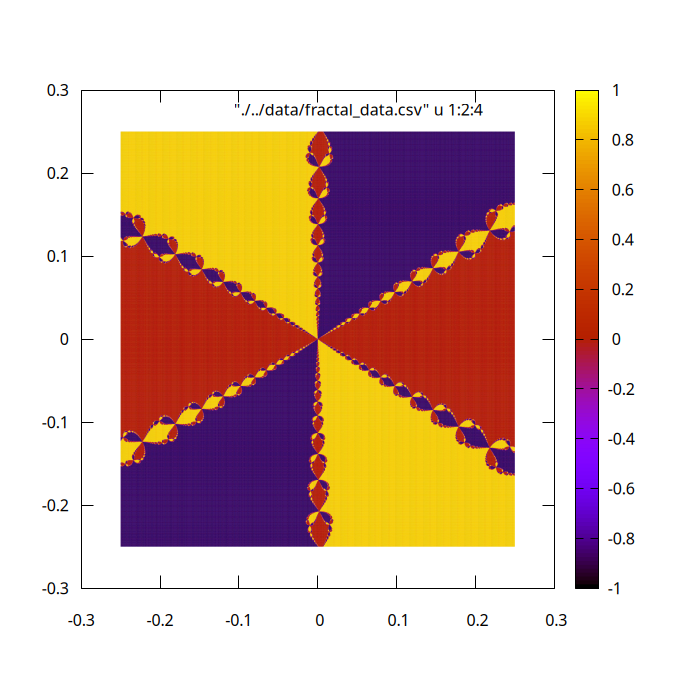
\includegraphics[width=0.75\textwidth]{./../problem04/plots/fractal_plot-02_02.png}
    \label{fig:02_02}
\end{figure}

     \begin{figure}[ht]
    \centering
    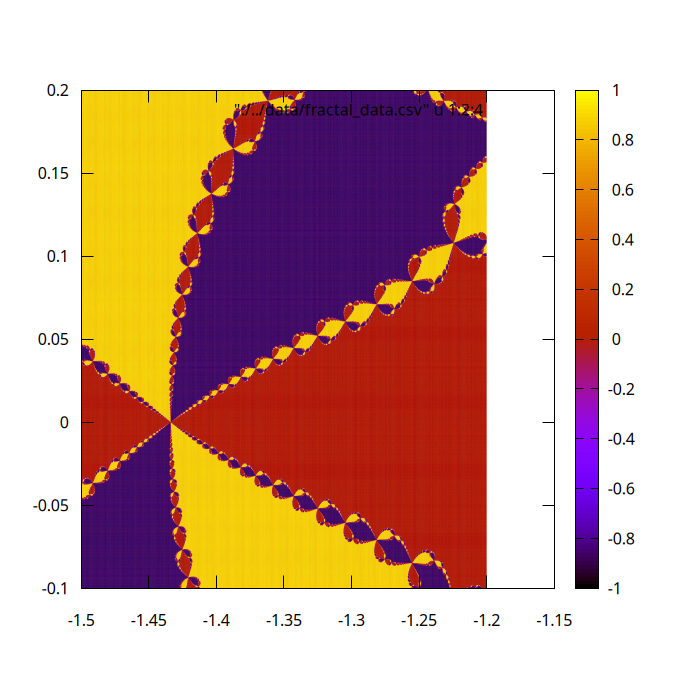
\includegraphics[width=0.75\textwidth]{./../problem04/plots/fractal_plot-02_03.png}
    \label{fig:02_03}
\end{figure}

After observing these intersting regions, we procede by plotting the number of iterations on the complex plane, zooming into locations with intersting behavior. 

     \begin{figure}[ht]
    \centering
    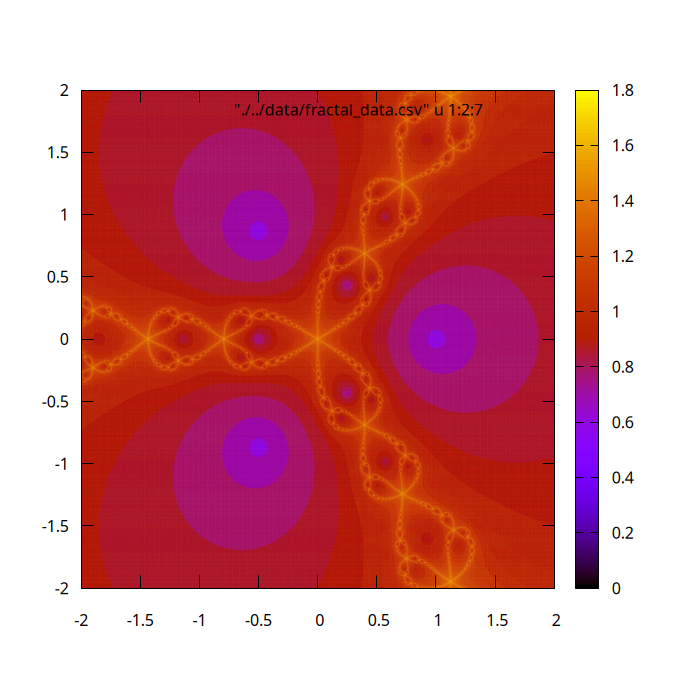
\includegraphics[width=0.75\textwidth]{./../problem04/plots/fractal_plot-02_05_iter.png}
    \label{fig:02_05}
\end{figure}
     \begin{figure}[ht]
    \centering
    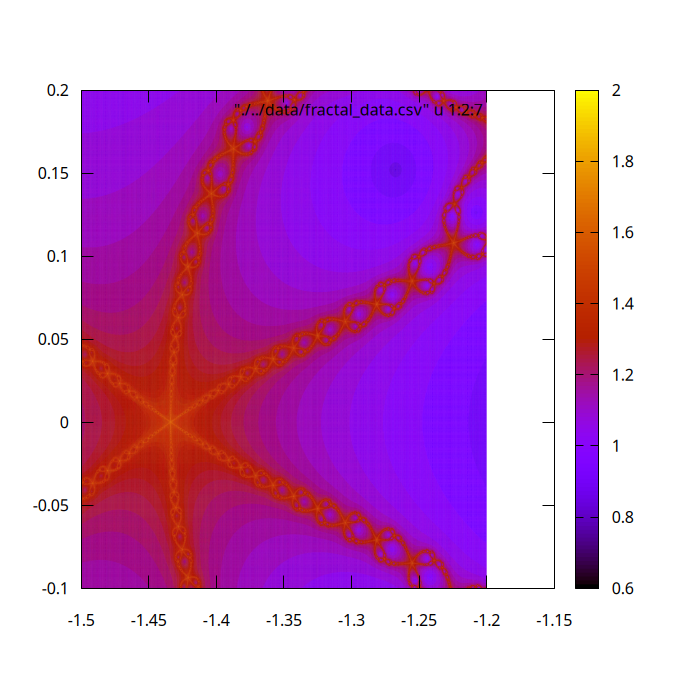
\includegraphics[width=0.75\textwidth]{./../problem04/plots/fractal_plot-02_04_iter.png}
    \label{fig:02_04}
\end{figure}
     \begin{figure}[ht]
    \centering
    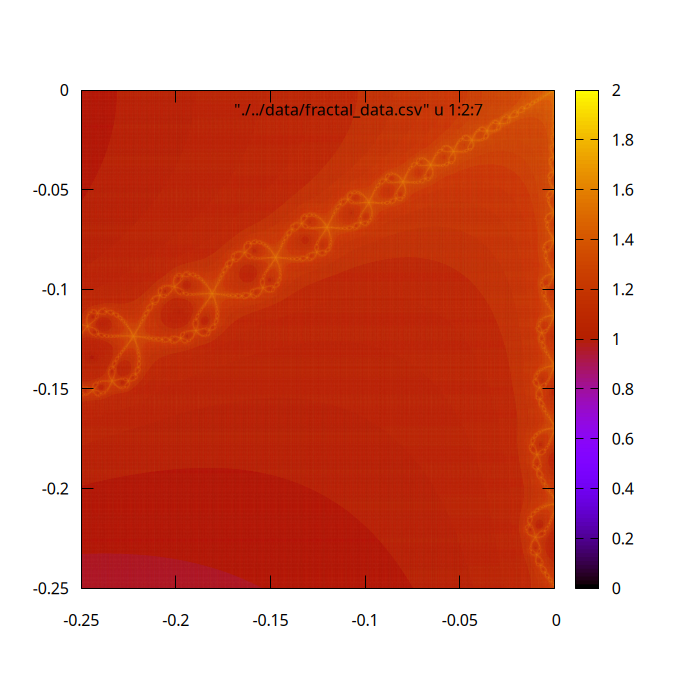
\includegraphics[width=0.75\textwidth]{./../problem04/plots/fractal_plot-02_06_iter.png}
    \label{fig:02_06}
\end{figure}

As we can see upon closer examination of the complex areas in the plot, there are not only single points that need greater iteration times, but even the local areas require more computation to finding a converging answer. This can be seen by the shifting of the colors and even the scales as one zooms further into the image. 

\subsection{Second Function}
\label{subsec:second}

We further continue the exercise by examining a second function given as follows:
\begin{align*}
	f \rb*{z} & =  35 z^{9} - 180 z^{7} + 378 z^{5} - 420 z^{3} + 315 z &\\
\end{align*}

This function shows more complex behavior and even regions in which the program was not able to converge to a root (resulting in me troubleshooting overflows). 

     \begin{figure}[ht]
    \centering
    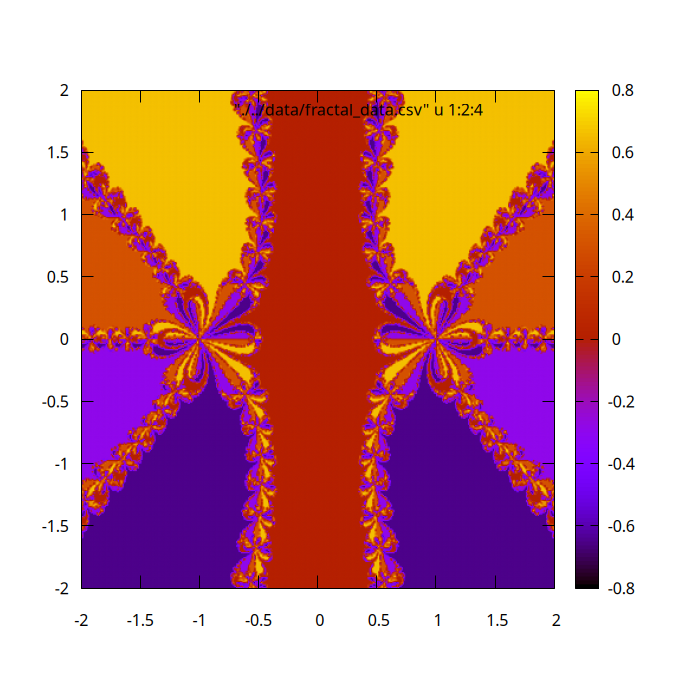
\includegraphics[width=0.75\textwidth]{./../problem04/plots/fractal_plot-03_01.png}
    \label{fig:03_01}
\end{figure}
     \begin{figure}[ht]
    \centering
    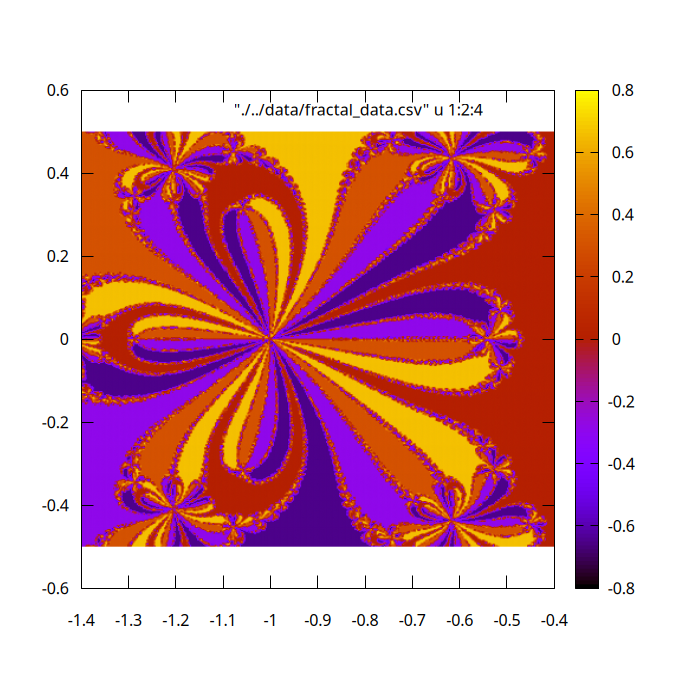
\includegraphics[width=0.75\textwidth]{./../problem04/plots/fractal_plot-03_02.png}
    \label{fig:03_02}

And we finish the assignment by examining the covergence plot of this function.
\end{figure}
     \begin{figure}[ht]
    \centering
    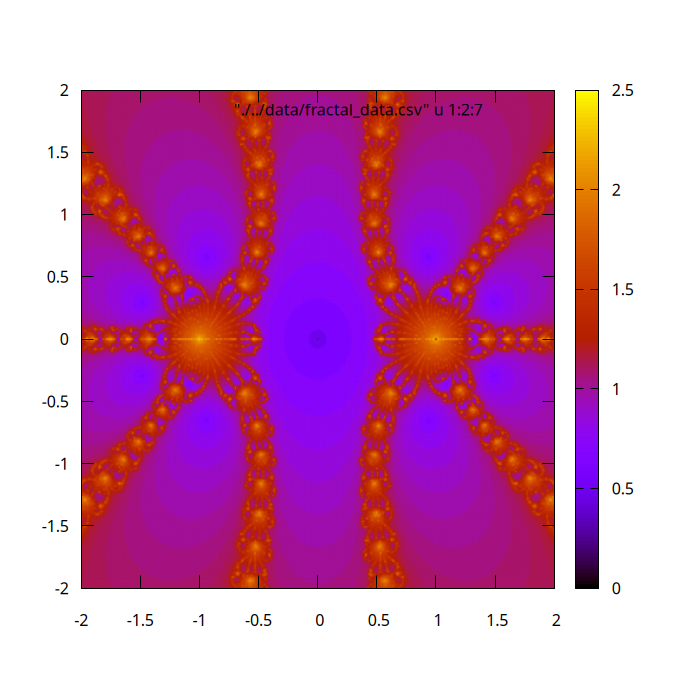
\includegraphics[width=0.75\textwidth]{./../problem04/plots/fractal_plot-03_03_iter.png}
    \label{fig:03_03}
\end{figure}
     \begin{figure}[ht]
    \centering
    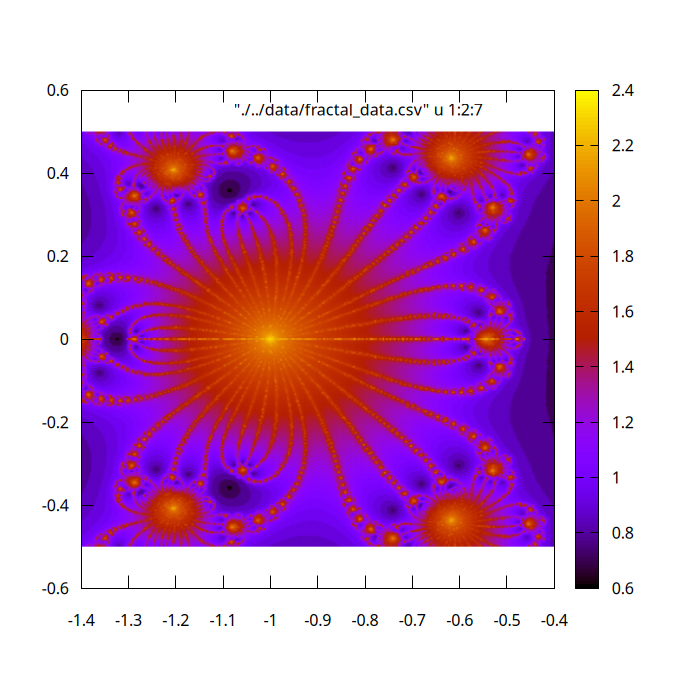
\includegraphics[width=0.75\textwidth]{./../problem04/plots/fractal_plot-03_04_iter.png}
    \label{fig:03_04}
\end{figure}


\end{document}
